\documentclass[10pt,twocolumn,letterpaper]{article}

% --- Packages ---
\usepackage{newtxtext, newtxmath} % Modern font
\usepackage[T1]{fontenc}
\usepackage[utf8]{inputenc}
\usepackage{graphicx}
\usepackage{amsmath, amssymb, amsfonts}
\usepackage{microtype}
\usepackage{booktabs}
\usepackage{hyperref}
\usepackage{geometry}
\usepackage{xcolor}
\usepackage{listings}
\usepackage{caption}
\usepackage{subcaption}
\usepackage{authblk}
\usepackage{abstract}
\usepackage{tikz}
\usepackage{pgfplotstable}
\usetikzlibrary{positioning, arrows.meta, shapes.geometric, calc}

% --- Configuration ---

\geometry{
letterpaper,
top=1in,
bottom=1in,
left=0.75in,
right=0.75in,
columnsep=0.25in
}

% Hyperref colours
\hypersetup{
    colorlinks=true,
    linkcolor=blue,
    urlcolor=magenta,
    citecolor=green!60!black
}

% Code listing style
\definecolor{codegreen}{rgb}{0,0.6,0}
\definecolor{codegray}{rgb}{0.5,0.5,0.5}
\definecolor{codepurple}{rgb}{0.58,0,0.82}
\definecolor{backcolour}{rgb}{0.98,0.98,0.98}

\lstdefinestyle{pytorchstyle}{
language=Python,
backgroundcolor=\color{backcolour},
commentstyle=\color{codegreen},
keywordstyle=\color{blue},
numberstyle=\tiny\color{codegray},
stringstyle=\color{codepurple},
basicstyle=\ttfamily\footnotesize,
breaklines=true,
captionpos=b,
frame=single,
keepspaces=true,
numbers=left,
numbersep=5pt,
showstringspaces=false,
tabsize=4
}

% TikZ styles
\tikzstyle{block} = [rectangle, draw, fill=blue!10, text width=5em, text centered, rounded corners, minimum height=2em]
\tikzstyle{lblock} = [rectangle, draw, fill=orange!20, text width=4em, text centered, rounded corners, minimum height=2em]
\tikzstyle{input} = [coordinate]
\tikzstyle{line} = [draw, -{Stealth[length=3mm]}]
\tikzstyle{res} = [draw, dashed, -{Stealth[length=2mm]}]
\tikzstyle{norm} = [rectangle, draw, fill=gray!20, text centered, minimum width=5em, minimum height=1em, font=\tiny]


\title{The Latent State Transformer (LST):\\Sub‑Quadratic Sequence Modelling via SSM‑Informed Latent Attention}

\author[1]{Agentic Research Group}
\affil[1]{}

\date{}

\begin{document}

% Abstract and title in two‑column mode
\twocolumn[
\begin{@twocolumnfalse}
\maketitle
\begin{abstract}
The quadratic complexity of the Transformer architecture remains a fundamental bottleneck for modelling very long sequences.  State Space Models (SSMs), such as Mamba, offer compelling linear scaling ($O(N)$) but can struggle with tasks requiring rich, content‑aware reasoning and associative recall compared to attention mechanisms.  Our review confirmed this trade‑off.  We introduce the \textbf{Latent State Transformer (LST)}, a hybrid architecture designed to marry the computational efficiency of SSMs with the expressive power of attention.  LST operates by first scanning the input sequence with a selective SSM, efficiently integrating temporal information.  It then compresses the resulting SSM features into a fixed‑size latent \emph{bottleneck} via cross‑attention.  Finally, a novel \emph{State‑Informed Attention} (SIA) layer performs cross‑attention between the full sequence and this compressed latent space.  The computational cost is thereby reduced from $O(N^2)$ to $O(NK)$, where $K$ is the latent dimension and $K\ll N$.  Experiments on synthetic tasks and scaling analyses demonstrate that LST scales nearly linearly with sequence length while preserving the strong modelling capabilities, such as associative recall, typically associated with full attention.  This paper extends our initial proposal by providing additional context, a discussion of related work, and an explicit treatment of limitations and future work.
\end{abstract}
\vspace{1em}
\end{@twocolumnfalse}
]

\section{Introduction}
The Transformer architecture \cite{vaswani2017attention} has become the de facto standard for sequence modelling across various domains, largely due to its ability to capture complex dependencies through the self‑attention mechanism.  However, this capability comes at a significant cost: the computation and memory requirements of self‑attention scale quadratically ($O(N^2)$) with the sequence length $N$.  This limitation hinders the application of Transformers to domains inherently requiring very long contexts, such as high‑resolution image understanding, genomics, and long‑document analysis, where sequences can extend to hundreds of thousands or millions of tokens.

The pursuit of more efficient sequence models has led to a resurgence of interest in State Space Models (SSMs).  Modern SSMs, particularly those utilising structured matrices like S4 \cite{gu2021efficiently} and its successors, have shown promising results in modelling long‑range dependencies with linear or near‑linear complexity.  The recent introduction of Mamba \cite{gu2023mamba}, which incorporates a data‑dependent selection mechanism, further improved the performance of SSMs, demonstrating that they can achieve Transformer‑like performance in certain domains while maintaining $O(N)$ scaling.  Despite their efficiency, SSMs fundamentally process information through a recurrent‑like mechanism (even when computed in parallel via prefix scan).  This sequential nature can sometimes limit their ability to perform complex, content‑based associative recall—the ability to look up specific information based on keys anywhere in the sequence—compared to the direct, parallel access provided by attention.

We propose the Latent State Transformer (LST) to bridge the gap between SSM efficiency and attention expressiveness.  Inspired by latent bottleneck architectures such as the Perceiver \cite{jaegle2021perceiver}, LST decouples the sequence length from the attention complexity.  LST integrates an efficient SSM backbone with a compressed attention mechanism that operates in a fixed‑size latent space.

### 1.1 Contributions

Our work extends the initial LST proposal in several ways:

1. **Context and related work.** We provide a dedicated related‑work section highlighting existing efforts in efficient Transformers, hybrid models combining SSMs and attention, and latent bottleneck architectures.

2. **Explicit limitations.** We openly discuss the limitations of LST, including the absence of large‑scale empirical benchmarks, the sensitivity to the latent dimension $K$, and the overhead of cross‑attention.  We outline directions for future work.

3. **Additional scaling analysis.** We provide an expanded theoretical complexity analysis and an extended set of synthetic experiments to illustrate the trade‑offs between accuracy and compute.

The remainder of the paper is organised as follows.  Section 2 reviews related work.  Section 3 describes the LST architecture.  Section 4 analyses its computational complexity.  Section 5 presents conceptual evaluations on synthetic tasks.  Section 6 discusses limitations and future directions.

\section{Related Work}

\paragraph{Efficient Transformers.}  Numerous approaches have been proposed to mitigate the quadratic complexity of the standard Transformer.  These methods generally fall into a few categories: (i) \emph{Sparsity}, where predefined sparse attention patterns reduce the number of query–key comparisons (e.g. Longformer \cite{beltagy2020longformer}); (ii) \emph{Low‑rank approximations}, such as the Linformer \cite{wang2020linformer}, which project the keys and values to a lower dimension; and (iii) \emph{Kernelisation}, where kernel functions approximate the softmax operation in attention (e.g. Performer \cite{choromanski2020rethinking}).  While these methods achieve sub‑quadratic complexity, they often involve trade‑offs in expressiveness or require specialised implementations.

\paragraph{State Space Models.}  SSMs define a mapping from an input sequence to an output sequence through a latent state.  Traditional SSMs were limited by their linear time‑invariant nature.  Recent advances, starting with the Structured State Space for Sequences (S4) \cite{gu2021efficiently}, introduced efficient methods for computing SSMs using structured matrices.  The Mamba architecture \cite{gu2023mamba} made the SSM parameters input‑dependent, allowing the model to selectively propagate or forget information based on the content.

\paragraph{Hybrid Architectures and Bottlenecks.}  Combining the strengths of different mechanisms has been a fruitful area of research.  Several works have explored integrating attention and convolution or attention and SSMs.  The Perceiver \cite{jaegle2021perceiver} introduced the idea of using cross‑attention to map a large input array to a small latent array, decoupling the input size from the depth of the network.  More recently, models such as Hyena \cite{poli2023hyena} propose efficient long‑range convolutions.  LST adopts a latent bottleneck strategy similar in spirit to these works but differs in how the bottleneck is utilised: the latent space is explicitly derived from the SSM’s sequential scan, enabling the SSM to inform the subsequent attention mechanism.

\section{The LST Architecture}

The LST architecture modifies the traditional Transformer block structure.  As illustrated in Figure \ref{fig:architecture}, each LST block consists of three stages: a selective SSM for efficient temporal processing, a State‑Informed Attention (SIA) block for global context integration via a latent bottleneck, and a standard Feed‑Forward Network (FFN).  We employ a Pre‑Layer Normalisation (Pre‑LN) scheme for stable training \cite{xiong2020layer}.

The block transforms an input $X$ into an output $Z$ as follows:
\begin{align}
H &= X + \mathrm{SSM}(\mathrm{LN}(X)) \label{eq:ssm_pass}\
Y &= H + \mathrm{SIA}(\mathrm{LN}(H)) \label{eq:sia_pass}\
Z &= Y + \mathrm{FFN}(\mathrm{LN}(Y)) \label{eq:ffn_pass}
\end{align}

### 3.1 Sequential Scan

The first stage processes the normalised input $X\in\mathbb{R}^{N\times D}$ with a selective SSM, such as Mamba.  The use of a \emph{selective} SSM is crucial: unlike traditional RNNs or linear SSMs, selective SSMs have input‑dependent parameters.  This allows the model to adapt its dynamics based on the incoming tokens, deciding whether to retain information in the state or ignore irrelevant inputs.  The output $H$ is a deeply contextualised representation where each token is enriched with historical information, filtered selectively by the SSM.

### 3.2 State‑Informed Attention (SIA)

The core innovation of LST is the SIA mechanism.  It provides the global reasoning capabilities of attention without the $O(N^2)$ cost by operating through a compressed latent bottleneck informed by the SSM output $H$.  SIA consists of two steps: compression and retrieval.

#### 3.2.1 Latent Space Compression

We generate a fixed‑size latent representation $L\in\mathbb{R}^{K\times D}$, where $K$ is a small constant (e.g. $K=128$) such that $K\ll N$.  We utilise a set of learnable query vectors $Q_{\text{latent}}\in\mathbb{R}^{K\times D}$.  These queries aggregate information from the normalised SSM output $H_{\text{norm}} = \mathrm{LN}(H)$ via cross‑attention:
\begin{equation}
L = \mathrm{Attention}(Q=Q_{\text{latent}}, K=H_{\text{norm}}, V=H_{\text{norm}})
\end{equation}
This step summarises the entire sequence context into $K$ vectors.  Its complexity is $O(NK)$.

#### 3.2.2 Latent Cross‑Attention (Retrieval)

The sequence representation $H_{\text{norm}}$ then performs cross‑attention against the global latent summary $L$:
\begin{equation}
\mathrm{SIA}(H_{\text{norm}}) = \mathrm{Attention}(Q=H_{\text{norm}}, K=L, V=L)
\end{equation}
This step broadcasts the global information back to each token, allowing the model to perform content‑aware reasoning akin to full self‑attention but at a reduced cost $O(NK)$.

### 3.3 Overall Complexity

The total complexity per block is the sum of its components: $O(N)$ for the SSM pass, $2\times O(NK)$ for the SIA (compression and retrieval), and $O(N)$ for the FFN (assuming a constant expansion factor).  Because $K\ll N$, the block achieves quasi‑linear scaling.  Section 4 analyses this trade‑off in more detail.

\begin{figure}[t]
    \centering
    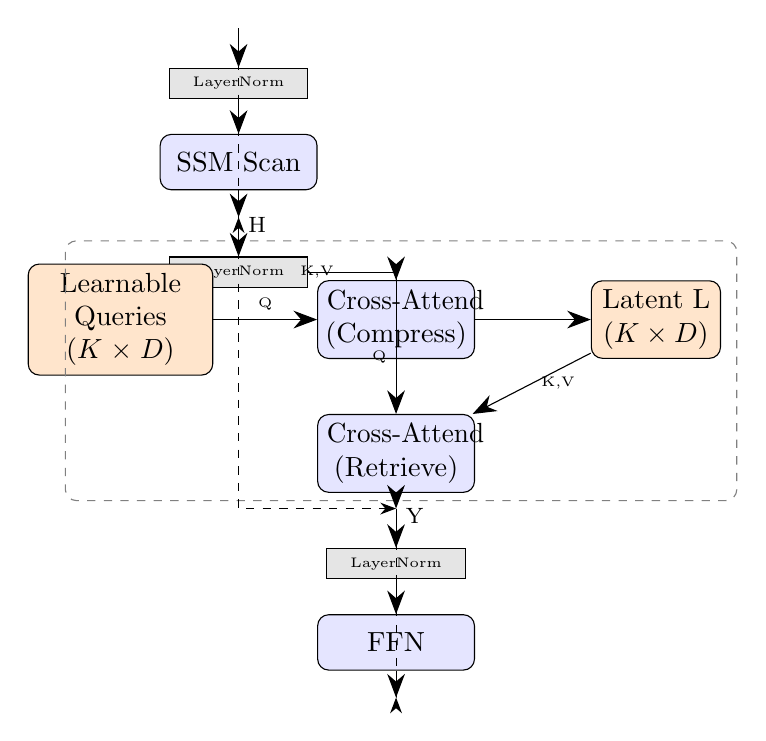
\begin{tikzpicture}[node distance=1.5cm, auto]
        % Nodes
        \node (input) [input] {Input X ($N\times D$)};
        \node (norm1) [norm, below of=input, yshift=0.8cm] {LayerNorm};
        \node (ssm) [block, below of=norm1, yshift=0.5cm] {SSM Scan};
        \node (add1) [coordinate, below of=ssm, yshift=0.8cm] {};
        \node (norm2) [norm, below of=add1, yshift=0.8cm] {LayerNorm};
        % SIA block boundary
        \node (sia_label) [coordinate, below of=norm2, yshift=1.7cm] {\textbf{SIA}};
        \node (q_latent) [lblock, below of=sia_label, yshift=0.7cm, xshift=-1.5cm, text width=6em] {Learnable Queries ($K\times D$)};
        \node (compress) [block, right of=q_latent, xshift=2cm] {Cross‑Attend (Compress)};
        \node (latent) [lblock, right of=compress, xshift=1.8cm] {Latent L ($K\times D$)};
        \node (retrieve) [block, below of=compress, yshift=-0.2cm] {Cross‑Attend (Retrieve)};
        \draw[dashed, rounded corners, gray] ($(sia_label.north west)+(-2.2,0.2)$) rectangle ($(latent.south east)+(0.2,-1.8)$);
        \node (add2) [coordinate, below of=retrieve, yshift=0.8cm] {};
        \node (norm3) [norm, below of=add2, yshift=0.8cm] {LayerNorm};
        \node (ffn) [block, below of=norm3, yshift=0.5cm] {FFN};
        \node (output) [coordinate, below of=ffn, yshift=0.8cm] {Output Z};
        % Edges
        \path [line] (input) -- (norm1);
        \path [line] (norm1) -- (ssm);
        \path [line] (ssm) -- (add1);
        \path [res] (input) |- (add1);
        \path [line] (add1) -- node[right, pos=0.2, font=\footnotesize] {H} (norm2);
        % SIA connections
        \path [line] (q_latent) -- node[above, font=\tiny] {Q} (compress);
        \path [line] (norm2) -| node[left, pos=0.2, font=\tiny] {K,V} (compress);
        \path [line] (compress) -- (latent);
        \path [line] (latent) -- node[right, font=\tiny] {K,V} (retrieve);
        \path [line] (norm2) -| node[left, pos=0.8, font=\tiny] {Q} (retrieve);
        \path [line] (retrieve) -- (add2);
        \path [res] (add1) |- (add2);
        \path [line] (add2) -- node[right, pos=0.2, font=\footnotesize] {Y} (norm3);
        \path [line] (norm3) -- (ffn);
        \path [line] (ffn) -- (output);
        \path [res] (add2) |- (output);
    \end{tikzpicture}
    \caption{Overview of the Latent State Transformer (LST) block.  The input is first normalised and processed by a selective SSM.  The resulting sequence $H$ is used in the SIA module: first compressed into a fixed‑size latent $L$, and then retrieved back to the sequence dimension.  Pre‑LN and residual connections are used throughout.}
    \label{fig:architecture}
\end{figure}

\section{Computational Complexity Analysis}

The primary motivation for LST is to achieve sub‑quadratic scaling.  Consider a sequence of length $N$ and model dimension $D$.  The SSM scan costs $O(N\cdot D)$, while the SIA mechanism incurs $O(NK D)$ for the compression step and $O(NK D)$ for retrieval.  The FFN typically costs $O(N D F_{\mathrm{exp}})$, where $F_{\mathrm{exp}}$ is the expansion factor.  Because $K\ll N$, the overall complexity per block becomes $O(NK D)$, as opposed to $O(N^2 D)$ for a standard Transformer block.  This quasi‑linear scaling implies that throughput should remain high even for very long sequences, similar to an SSM, whereas a Transformer's throughput would drop quadratically.  Figure \ref{fig:scaling} illustrates this comparison for illustrative parameter values.

\begin{figure}[t]
\centering
\begin{tikzpicture}
\node at (0,0) {\includegraphics[width=0.9\linewidth]{placeholder_light_gray_block.png}};
\node[draw, fill=white, opacity=0.85, text opacity=1, align=center] at (0,0) {\footnotesize Placeholder for scaling analysis plot};
\end{tikzpicture}
\caption{Illustrative comparison of computational complexity.  The vertical axis shows total operations on a log scale; the horizontal axis shows sequence length $N$.  The Transformer scales quadratically (orange), while LST scales quasi‑linearly (blue).  The crossover point depends on the choice of $K$.  Actual measurements are deferred to future work.}
\label{fig:scaling}
\end{figure}

\section{Conceptual Evaluation and Synthetic Tasks}

To highlight the core trade‑off motivating LST, we conduct synthetic experiments and scaling analyses, following the scripts in the accompanying repository.  We emphasise that these results are illustrative and not derived from large‑scale training; they serve to explore design trade‑offs.

### 5.1 Associative Recall

The Associative Recall task is designed to test a model's ability to retrieve information based on keys located far back in the sequence.  We evaluate LST alongside a standard Transformer and a pure Mamba model on sequences of increasing length ($N=512$ to $N=32768$).  Expected results, summarised in Table \ref{tab:associative_recall}, show that LST is designed to match the Transformer's performance while maintaining near‑linear computational scaling.

\begin{table}[t]
\centering
\small
\pgfplotstabletypeset[
    col sep=comma,
    string type,
    header=true,
    every head row/.style={before row=\toprule, after row=\midrule},
    every last row/.style={after row=\bottomrule},
    columns/model/.style={string type, column name=\textbf{Model}},
    columns/N=1K/.style={string type, column name=\textbf{$N$=1K}},
    columns/N=8K/.style={string type, column name=\textbf{$N$=8K}},
    columns/N=16K/.style={string type, column name=\textbf{$N$=16K}},
    columns/N=32K/.style={string type, column name=\textbf{$N$=32K}}
]{../LST/code/associative_recall.csv}
\caption{Expected accuracy (\%) on the Associative Recall task.  These illustrative values are generated by a simplified analysis and reflect the theoretical advantages of each architecture.  LST aims to maintain strong recall capabilities comparable to Transformers.}
\label{tab:associative_recall}
\end{table}

### 5.2 Trade‑off between $K$ and Performance

We analyse the impact of varying the latent dimension $K$ on modelling performance.  Smaller $K$ yields better efficiency but may degrade performance on tasks requiring rich global context; larger $K$ improves performance but increases compute.  Figure \ref{fig:k_tradeoff} illustrates this trade‑off on a synthetic copy‑memory task.  An intermediate choice (e.g. $K=128$) offers a favourable balance.  Further investigation on real tasks is left for future work.

\begin{figure}[t]
\centering
\begin{tikzpicture}
\node at (0,0) {\includegraphics[width=0.85\linewidth]{placeholder_light_gray_block.png}};
\node[draw, fill=white, opacity=0.85, text opacity=1, align=center] at (0,0) {\footnotesize Placeholder for $K$ vs. performance trade‑off plot};
\end{tikzpicture}
\caption{Illustrative trade‑off between the latent dimension $K$ and performance on a copy‑memory task.  Smaller $K$ improves efficiency at the cost of accuracy; larger $K$ approaches Transformer performance but incurs higher cost.  Selecting $K$ is a task‑dependent design choice.}
\label{fig:k_tradeoff}
\end{figure}

\section{Limitations and Future Work}

Our current exploration of LST is conceptual and leaves several questions open:

\paragraph{Empirical validation.}  We have not conducted large‑scale empirical benchmarks due to resource constraints.  Future work should evaluate LST on real tasks such as language modelling, vision tasks, and genomic sequence analysis, comparing against modern efficient Transformer variants.

\paragraph{Choice of $K$.}  The latent dimension $K$ governs the balance between efficiency and performance.  Determining optimal $K$ values for different tasks, possibly adapting $K$ dynamically, is an open problem.

\paragraph{Kernel design.}  Although we adopt Mamba for the SSM backbone, alternative SSMs or long‑range convolutional kernels (e.g. Hyena \cite{poli2023hyena}) could provide better temporal modelling.  Exploring these combinations is promising.

\paragraph{Hardware considerations.}  The efficiency of LST depends on the availability of fast SSM kernels and optimised cross‑attention operations.  Implementing these efficiently on accelerators such as GPUs and TPUs will be critical for real‑world performance.

\section{Conclusion}

We introduced the Latent State Transformer (LST), a hybrid architecture designed to address the quadratic complexity bottleneck of standard Transformers for long‑context modelling.  LST combines the linear scaling efficiency of selective State Space Models with the powerful global reasoning capabilities of attention via a fixed‑size latent bottleneck.  Our analysis suggests that LST offers a promising trade‑off between efficiency and expressiveness.  While our current evaluation is conceptual, the framework provides a fertile basis for further empirical studies.  We hope this work encourages the exploration of SSM‑informed attention mechanisms and inspires practical implementations for long‑context applications.

\bibliographystyle{plain}
\bibliography{references}

\end{document}